% Options for packages loaded elsewhere
\PassOptionsToPackage{unicode}{hyperref}
\PassOptionsToPackage{hyphens}{url}
%
\documentclass[
  english,
  ,doc,floatsintext]{apa6}
\usepackage{lmodern}
\usepackage{amssymb,amsmath}
\usepackage{ifxetex,ifluatex}
\ifnum 0\ifxetex 1\fi\ifluatex 1\fi=0 % if pdftex
  \usepackage[T1]{fontenc}
  \usepackage[utf8]{inputenc}
  \usepackage{textcomp} % provide euro and other symbols
\else % if luatex or xetex
  \usepackage{unicode-math}
  \defaultfontfeatures{Scale=MatchLowercase}
  \defaultfontfeatures[\rmfamily]{Ligatures=TeX,Scale=1}
\fi
% Use upquote if available, for straight quotes in verbatim environments
\IfFileExists{upquote.sty}{\usepackage{upquote}}{}
\IfFileExists{microtype.sty}{% use microtype if available
  \usepackage[]{microtype}
  \UseMicrotypeSet[protrusion]{basicmath} % disable protrusion for tt fonts
}{}
\makeatletter
\@ifundefined{KOMAClassName}{% if non-KOMA class
  \IfFileExists{parskip.sty}{%
    \usepackage{parskip}
  }{% else
    \setlength{\parindent}{0pt}
    \setlength{\parskip}{6pt plus 2pt minus 1pt}}
}{% if KOMA class
  \KOMAoptions{parskip=half}}
\makeatother
\usepackage{xcolor}
\IfFileExists{xurl.sty}{\usepackage{xurl}}{} % add URL line breaks if available
\IfFileExists{bookmark.sty}{\usepackage{bookmark}}{\usepackage{hyperref}}
\hypersetup{
  pdftitle={Some exploration of Oxford Policy Response Database},
  hidelinks,
  pdfcreator={LaTeX via pandoc}}
\urlstyle{same} % disable monospaced font for URLs
\usepackage{color}
\usepackage{fancyvrb}
\newcommand{\VerbBar}{|}
\newcommand{\VERB}{\Verb[commandchars=\\\{\}]}
\DefineVerbatimEnvironment{Highlighting}{Verbatim}{commandchars=\\\{\}}
% Add ',fontsize=\small' for more characters per line
\usepackage{framed}
\definecolor{shadecolor}{RGB}{248,248,248}
\newenvironment{Shaded}{\begin{snugshade}}{\end{snugshade}}
\newcommand{\AlertTok}[1]{\textcolor[rgb]{0.94,0.16,0.16}{#1}}
\newcommand{\AnnotationTok}[1]{\textcolor[rgb]{0.56,0.35,0.01}{\textbf{\textit{#1}}}}
\newcommand{\AttributeTok}[1]{\textcolor[rgb]{0.77,0.63,0.00}{#1}}
\newcommand{\BaseNTok}[1]{\textcolor[rgb]{0.00,0.00,0.81}{#1}}
\newcommand{\BuiltInTok}[1]{#1}
\newcommand{\CharTok}[1]{\textcolor[rgb]{0.31,0.60,0.02}{#1}}
\newcommand{\CommentTok}[1]{\textcolor[rgb]{0.56,0.35,0.01}{\textit{#1}}}
\newcommand{\CommentVarTok}[1]{\textcolor[rgb]{0.56,0.35,0.01}{\textbf{\textit{#1}}}}
\newcommand{\ConstantTok}[1]{\textcolor[rgb]{0.00,0.00,0.00}{#1}}
\newcommand{\ControlFlowTok}[1]{\textcolor[rgb]{0.13,0.29,0.53}{\textbf{#1}}}
\newcommand{\DataTypeTok}[1]{\textcolor[rgb]{0.13,0.29,0.53}{#1}}
\newcommand{\DecValTok}[1]{\textcolor[rgb]{0.00,0.00,0.81}{#1}}
\newcommand{\DocumentationTok}[1]{\textcolor[rgb]{0.56,0.35,0.01}{\textbf{\textit{#1}}}}
\newcommand{\ErrorTok}[1]{\textcolor[rgb]{0.64,0.00,0.00}{\textbf{#1}}}
\newcommand{\ExtensionTok}[1]{#1}
\newcommand{\FloatTok}[1]{\textcolor[rgb]{0.00,0.00,0.81}{#1}}
\newcommand{\FunctionTok}[1]{\textcolor[rgb]{0.00,0.00,0.00}{#1}}
\newcommand{\ImportTok}[1]{#1}
\newcommand{\InformationTok}[1]{\textcolor[rgb]{0.56,0.35,0.01}{\textbf{\textit{#1}}}}
\newcommand{\KeywordTok}[1]{\textcolor[rgb]{0.13,0.29,0.53}{\textbf{#1}}}
\newcommand{\NormalTok}[1]{#1}
\newcommand{\OperatorTok}[1]{\textcolor[rgb]{0.81,0.36,0.00}{\textbf{#1}}}
\newcommand{\OtherTok}[1]{\textcolor[rgb]{0.56,0.35,0.01}{#1}}
\newcommand{\PreprocessorTok}[1]{\textcolor[rgb]{0.56,0.35,0.01}{\textit{#1}}}
\newcommand{\RegionMarkerTok}[1]{#1}
\newcommand{\SpecialCharTok}[1]{\textcolor[rgb]{0.00,0.00,0.00}{#1}}
\newcommand{\SpecialStringTok}[1]{\textcolor[rgb]{0.31,0.60,0.02}{#1}}
\newcommand{\StringTok}[1]{\textcolor[rgb]{0.31,0.60,0.02}{#1}}
\newcommand{\VariableTok}[1]{\textcolor[rgb]{0.00,0.00,0.00}{#1}}
\newcommand{\VerbatimStringTok}[1]{\textcolor[rgb]{0.31,0.60,0.02}{#1}}
\newcommand{\WarningTok}[1]{\textcolor[rgb]{0.56,0.35,0.01}{\textbf{\textit{#1}}}}
\usepackage{graphicx,grffile}
\makeatletter
\def\maxwidth{\ifdim\Gin@nat@width>\linewidth\linewidth\else\Gin@nat@width\fi}
\def\maxheight{\ifdim\Gin@nat@height>\textheight\textheight\else\Gin@nat@height\fi}
\makeatother
% Scale images if necessary, so that they will not overflow the page
% margins by default, and it is still possible to overwrite the defaults
% using explicit options in \includegraphics[width, height, ...]{}
\setkeys{Gin}{width=\maxwidth,height=\maxheight,keepaspectratio}
% Set default figure placement to htbp
\makeatletter
\def\fps@figure{htbp}
\makeatother
\setlength{\emergencystretch}{3em} % prevent overfull lines
\providecommand{\tightlist}{%
  \setlength{\itemsep}{0pt}\setlength{\parskip}{0pt}}
\setcounter{secnumdepth}{-\maxdimen} % remove section numbering
% Make \paragraph and \subparagraph free-standing
\ifx\paragraph\undefined\else
  \let\oldparagraph\paragraph
  \renewcommand{\paragraph}[1]{\oldparagraph{#1}\mbox{}}
\fi
\ifx\subparagraph\undefined\else
  \let\oldsubparagraph\subparagraph
  \renewcommand{\subparagraph}[1]{\oldsubparagraph{#1}\mbox{}}
\fi
% Manuscript styling
\usepackage{upgreek}
\captionsetup{font=singlespacing,justification=justified}

% Table formatting
\usepackage{longtable}
\usepackage{lscape}
% \usepackage[counterclockwise]{rotating}   % Landscape page setup for large tables
\usepackage{multirow}		% Table styling
\usepackage{tabularx}		% Control Column width
\usepackage[flushleft]{threeparttable}	% Allows for three part tables with a specified notes section
\usepackage{threeparttablex}            % Lets threeparttable work with longtable

% Create new environments so endfloat can handle them
% \newenvironment{ltable}
%   {\begin{landscape}\begin{center}\begin{threeparttable}}
%   {\end{threeparttable}\end{center}\end{landscape}}
\newenvironment{lltable}{\begin{landscape}\begin{center}\begin{ThreePartTable}}{\end{ThreePartTable}\end{center}\end{landscape}}

% Enables adjusting longtable caption width to table width
% Solution found at http://golatex.de/longtable-mit-caption-so-breit-wie-die-tabelle-t15767.html
\makeatletter
\newcommand\LastLTentrywidth{1em}
\newlength\longtablewidth
\setlength{\longtablewidth}{1in}
\newcommand{\getlongtablewidth}{\begingroup \ifcsname LT@\roman{LT@tables}\endcsname \global\longtablewidth=0pt \renewcommand{\LT@entry}[2]{\global\advance\longtablewidth by ##2\relax\gdef\LastLTentrywidth{##2}}\@nameuse{LT@\roman{LT@tables}} \fi \endgroup}

% \setlength{\parindent}{0.5in}
% \setlength{\parskip}{0pt plus 0pt minus 0pt}

% \usepackage{etoolbox}
\makeatletter
\patchcmd{\HyOrg@maketitle}
  {\section{\normalfont\normalsize\abstractname}}
  {\section*{\normalfont\normalsize\abstractname}}
  {}{\typeout{Failed to patch abstract.}}
\makeatother
\shorttitle{SHORTTITLE}
\author{Lionel\ \& Orestis}
\affiliation{\phantom{a}}
\usepackage{csquotes}
\usepackage{setspace, appendix, placeins}
\usepackage[justification=centering]{caption}
\usepackage{float}
\floatplacement{figure}{H}
\newcommand{\onote}[1]{{\color{blue} {(\sf orestis:} {\sl{#1}}     {\sf )}}}
\newcommand{\lnote}[1]{{\color{green} {(\sf lio:} {\sl{#1}}     {\sf )}}}
\newtheorem{finding}{Finding}
\ifxetex
  % Load polyglossia as late as possible: uses bidi with RTL langages (e.g. Hebrew, Arabic)
  \usepackage{polyglossia}
  \setmainlanguage[]{english}
\else
  \usepackage[shorthands=off,main=english]{babel}
\fi

\title{Some exploration of Oxford Policy Response Database}

\date{25 May, 2020}

\begin{document}
\maketitle

\hypertarget{comparison-with-coronanet}{%
\subsection{Comparison with CoronaNet}\label{comparison-with-coronanet}}

Simply plotting all observations from CoronaNet (CN) and the Oxford Database (Ox) reveals that, as expected, both are quite correlated (0.7), but the relationship is far from being perfect.

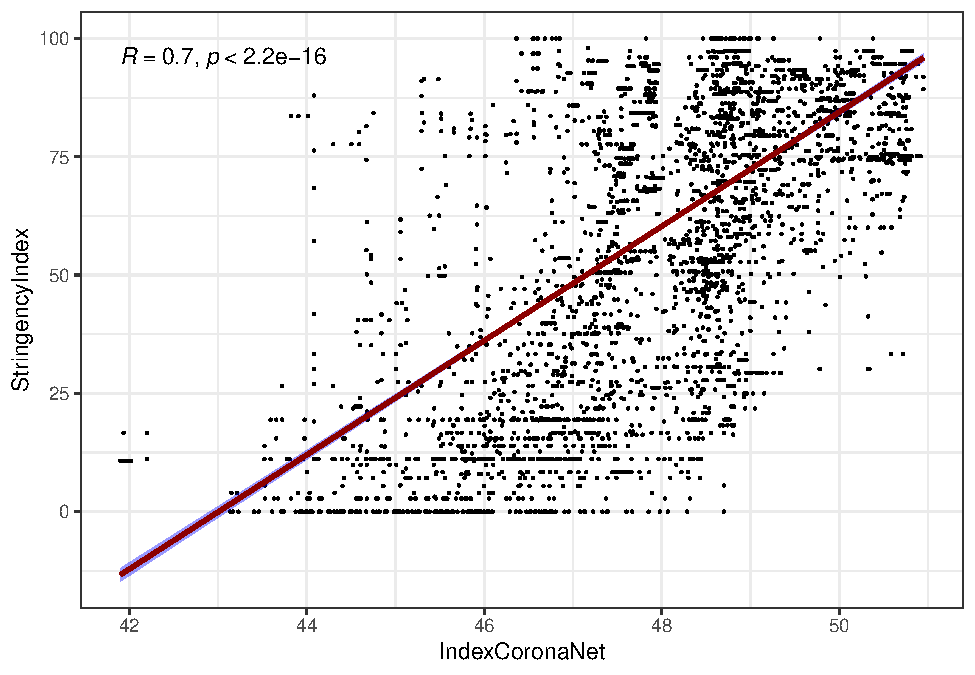
\includegraphics{LR_explore_OK_comms_files/figure-latex/scatter-1.pdf}

Illustrating this for a couple of (partly random) countries further shows where these differences stem from. A couple of things:

\begin{itemize}
\tightlist
\item
  CN starts at random periods, and often with odd values (suggesting quite strict policies at points in time where most likely no measures had been taken)

  \begin{itemize}
  \item
    {\color{blue} {(\sf orestis:} {\sl{Why is that?}}     {\sf )}}
  \end{itemize}
\item
  CN doesn't exhibit a line for US here, because it is federal and they report by state. Ox do the aggregation for us, whether this is to our satisfaction will have to be seen.
\item
  Easing of lockdowns seems to be hardly reflected in CN data, whereas Ox seems quite responsive.
\end{itemize}

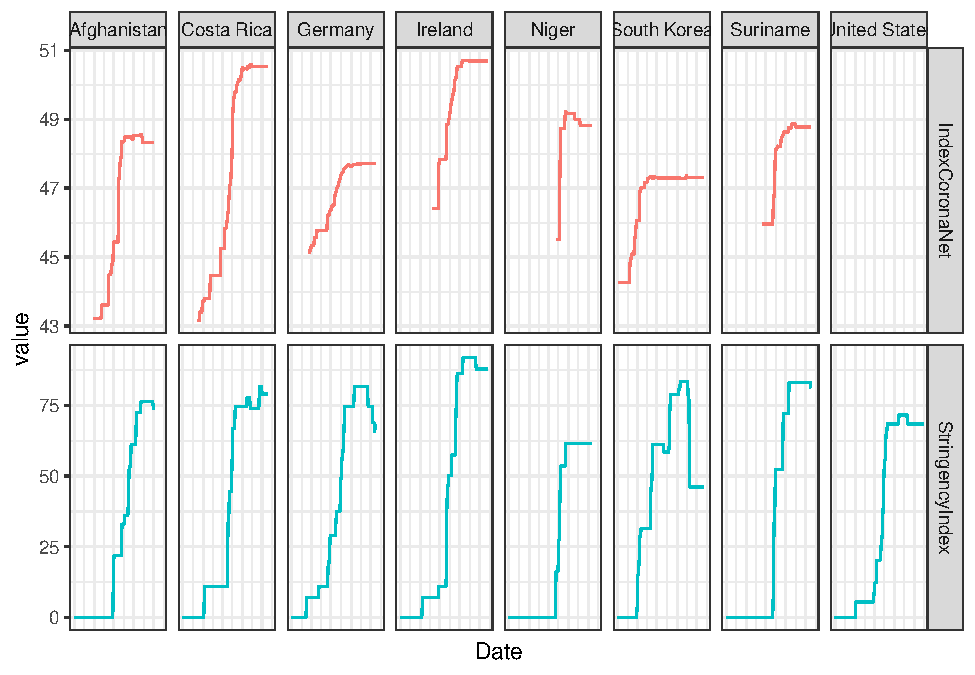
\includegraphics{LR_explore_OK_comms_files/figure-latex/lines compare-1.pdf}

Overall, it feels safe to assume that Ox is the better dataset to work with.

\hypertarget{plotting-duration-of-individual-measures}{%
\subsection{Plotting duration of individual measures}\label{plotting-duration-of-individual-measures}}

Ox comes with the neat \enquote{flag} variables, which are 1 if any given measure is in place and 0 otherwise (there is also the version that ranges 0-3 and says something about intensity).

The graph below is an attempt at depicting that information in a single graph, admittedly implemented in a slightly overcomplicated way (somewhat cheating ggplot)). The information content is quite high I find, I just wish I'd gone for a simpler approach (e.g.~seperate graphs for index and measures, line chart on top and bar chart / gantt chart below for each country). Also, that's why the legend is improvised.

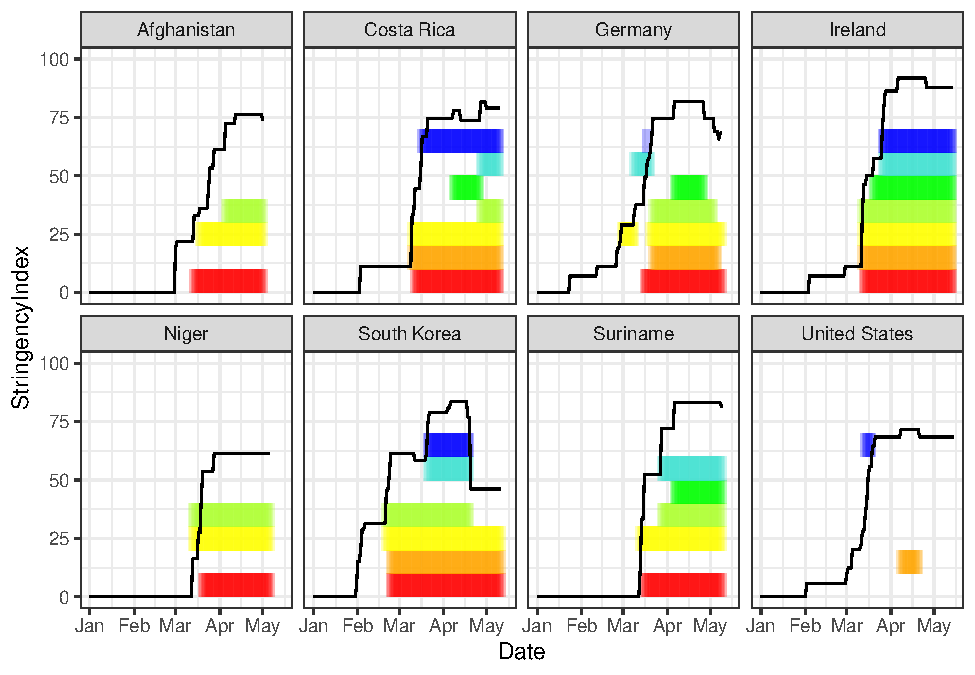
\includegraphics{LR_explore_OK_comms_files/figure-latex/measures-1.pdf}

\begin{figure}
\centering
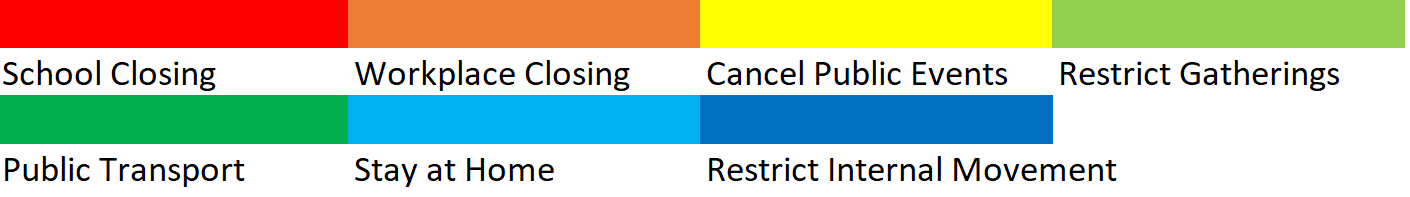
\includegraphics{legend_improvised.PNG}
\caption{legend}
\end{figure}

One take away is that, even in Ox, the US remains an odd case.

\hypertarget{estimating-compliance-using-ardl-model}{%
\subsection{Estimating compliance using ARDL model}\label{estimating-compliance-using-ardl-model}}

What follows is based on ARDL estimates, which is nothing but OLS where x (here: Movement) is explained with lags of x itself, as well as present values and lagged values of y (here: Stringency). Based on the obtained coefficients, it is easy to compute the \enquote{long run effect} of y on x, taking into account the feedback mechanisms that take place.

This should be a better way of quantifying \enquote{compliance}, as we don't have to make strong assumptions about which lag to use etc., and should some lag be more relevant than in others, this will not cause any issues.

Note that I am looking at differenced variables, as otherwise non-stationarity / spurious regression would certainly be an issue.

For example, the results for Zimbabwe read (*output seems to come out twice, don't know why):

\begin{verbatim}
## 
## Time series regression with "ts" data:
## Start = 4, End = 79
## 
## Call:
## dynlm(formula = as.formula(model.text), data = data)
## 
## Residuals:
##     Min      1Q  Median      3Q     Max 
## -36.770  -2.094  -0.100   2.646  21.800 
## 
## Coefficients:
##                        Estimate Std. Error t value Pr(>|t|)    
## (Intercept)              0.8366     1.0769   0.777  0.43995    
## diff.StringencyIndex.t  -1.0031     0.2227  -4.505 2.68e-05 ***
## diff.StringencyIndex.1  -0.1552     0.2569  -0.604  0.54779    
## diff.StringencyIndex.2  -0.4602     0.2562  -1.796  0.07687 .  
## diff.StringencyIndex.3  -0.4727     0.2605  -1.814  0.07403 .  
## diff.Movement.1         -0.3793     0.1196  -3.170  0.00229 ** 
## diff.Movement.2         -0.4080     0.1194  -3.417  0.00107 ** 
## diff.Movement.3         -0.2005     0.1211  -1.655  0.10248    
## ---
## Signif. codes:  0 '***' 0.001 '**' 0.01 '*' 0.05 '.' 0.1 ' ' 1
## 
## Residual standard error: 8.754 on 68 degrees of freedom
## Multiple R-squared:  0.4134, Adjusted R-squared:  0.3531 
## F-statistic: 6.847 on 7 and 68 DF,  p-value: 3.711e-06
\end{verbatim}

From these coefficients, the long-run effect can be derived using the formula sum({[}coefficients of y{]})/(1-sum(coefficients of x)). For Zim, this is -1.052: A 1 unit increase in stringency will lead to a 1.052\% decrease in Movement, in the long run.

The graphs below show coefficients for all countries, as well as by continent and geographical region. Low numbers mean high compliance.

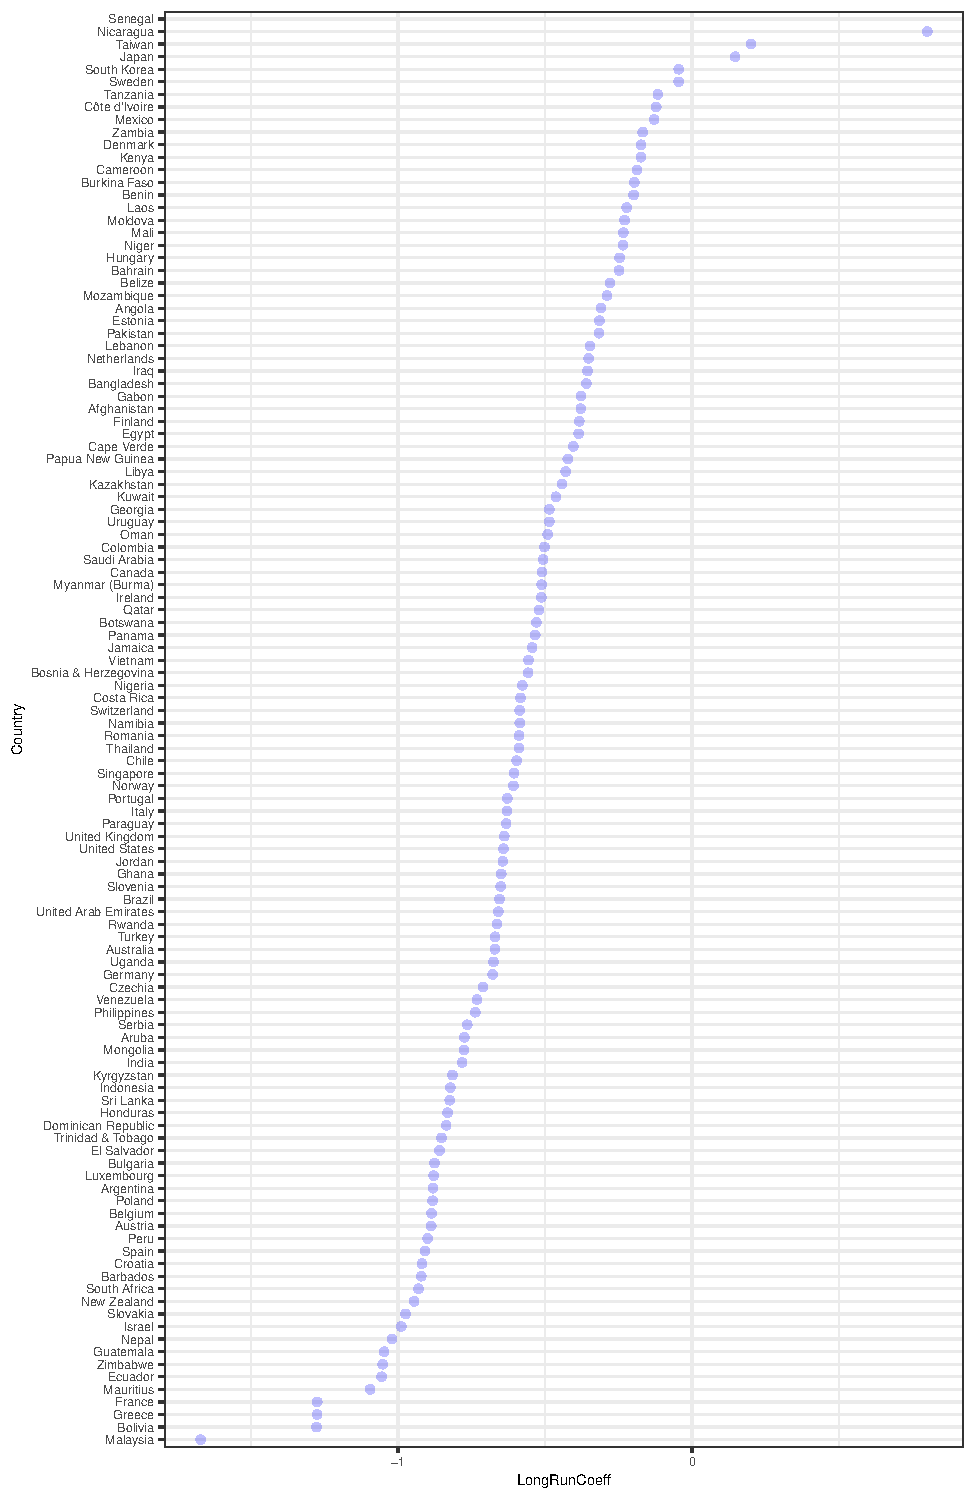
\includegraphics{LR_explore_OK_comms_files/figure-latex/coeff graphs-1.pdf}

Putting the previous figure into a table:

\begin{Shaded}
\begin{Highlighting}[]
\KeywordTok{datatable}\NormalTok{(lr.coeffs.covariates)}
\end{Highlighting}
\end{Shaded}

\hypertarget{htmlwidget-9b926721de3670c8b327}{}

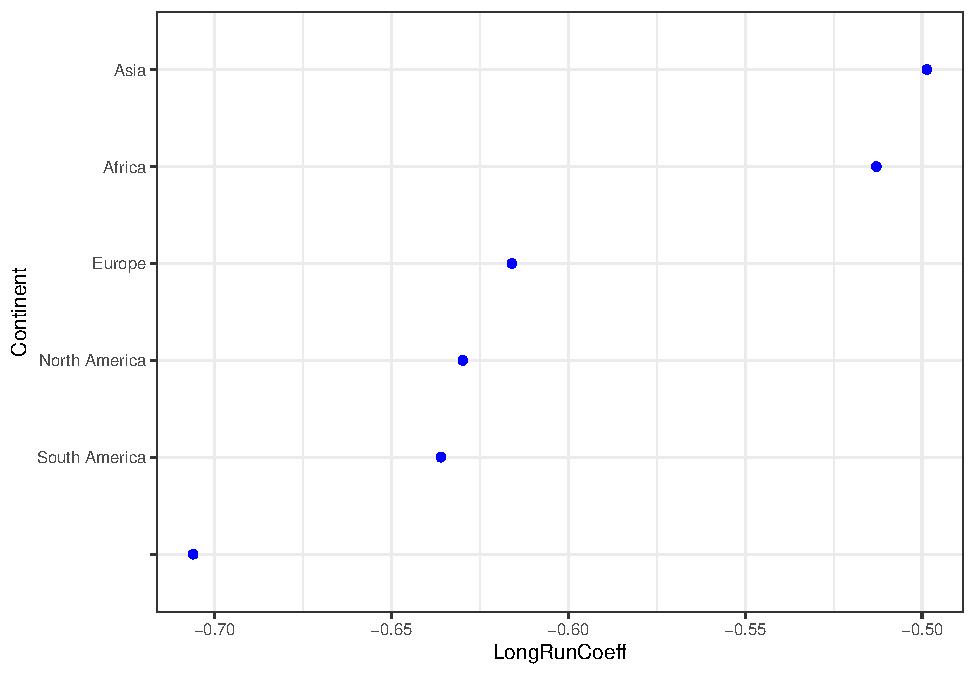
\includegraphics{LR_explore_OK_comms_files/figure-latex/coeffs by-1.pdf} 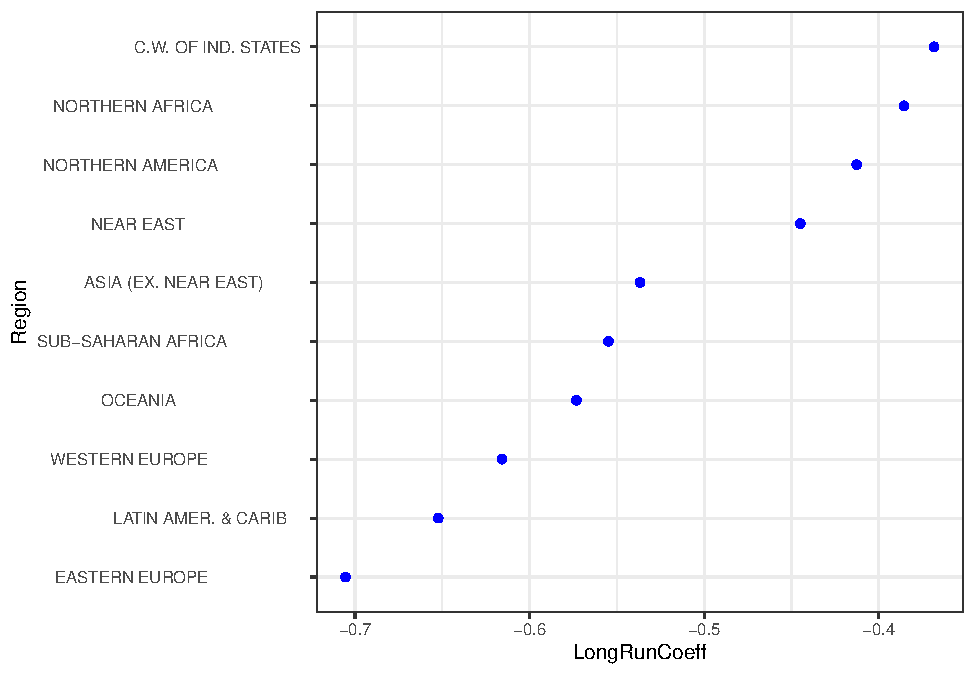
\includegraphics{LR_explore_OK_comms_files/figure-latex/coeffs by-2.pdf}

Asia being the \enquote{least} compliant is probably counterintuitive, but would be in line with targeted measures (*Korea remains a puzzle). Note also that China is not part of the sample as there's no Movement data.

\hypertarget{potential-determinants-covariates-of-compliance}{%
\subsection{Potential determinants / covariates of compliance}\label{potential-determinants-covariates-of-compliance}}

Below, as usual a couple of scatterplots plotting this measure of compliance against a number of other factors (see axis labels).

Spoiler: Nothing going on.

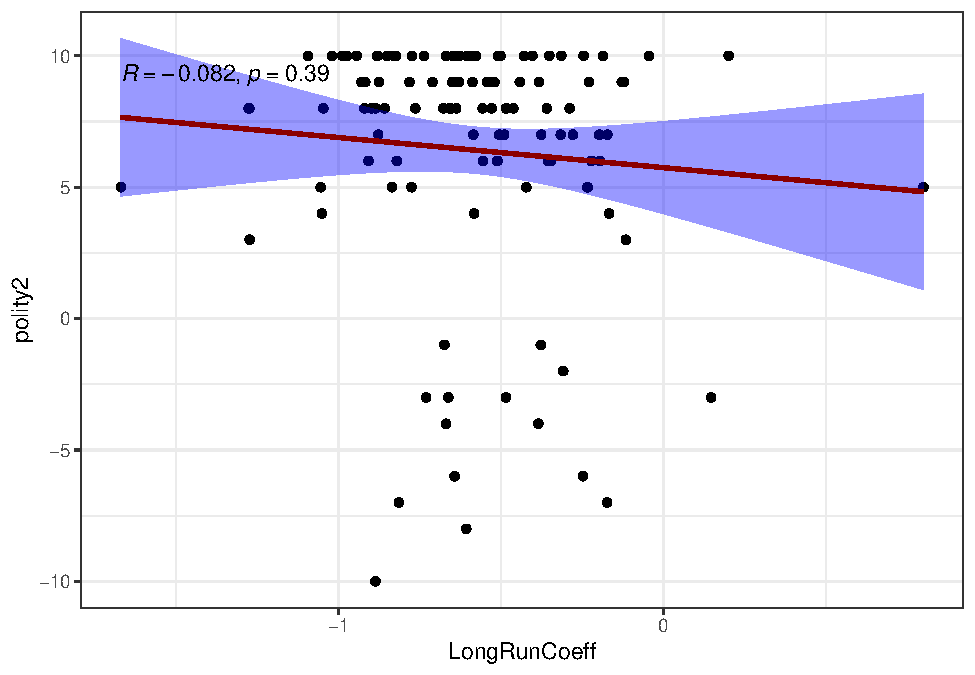
\includegraphics{LR_explore_OK_comms_files/figure-latex/covariates-1.pdf} 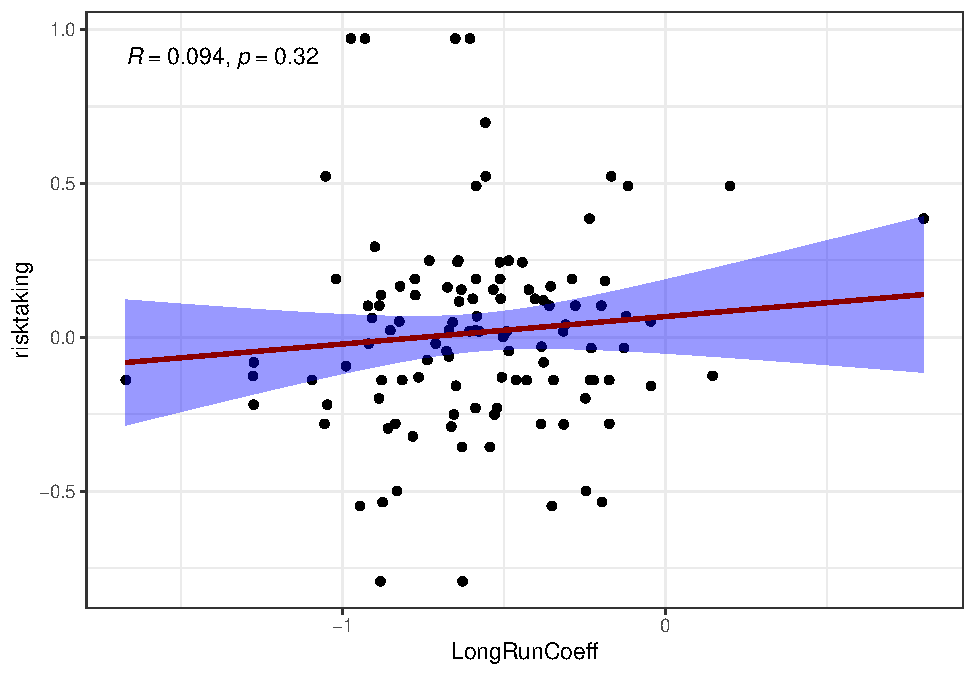
\includegraphics{LR_explore_OK_comms_files/figure-latex/covariates-2.pdf} 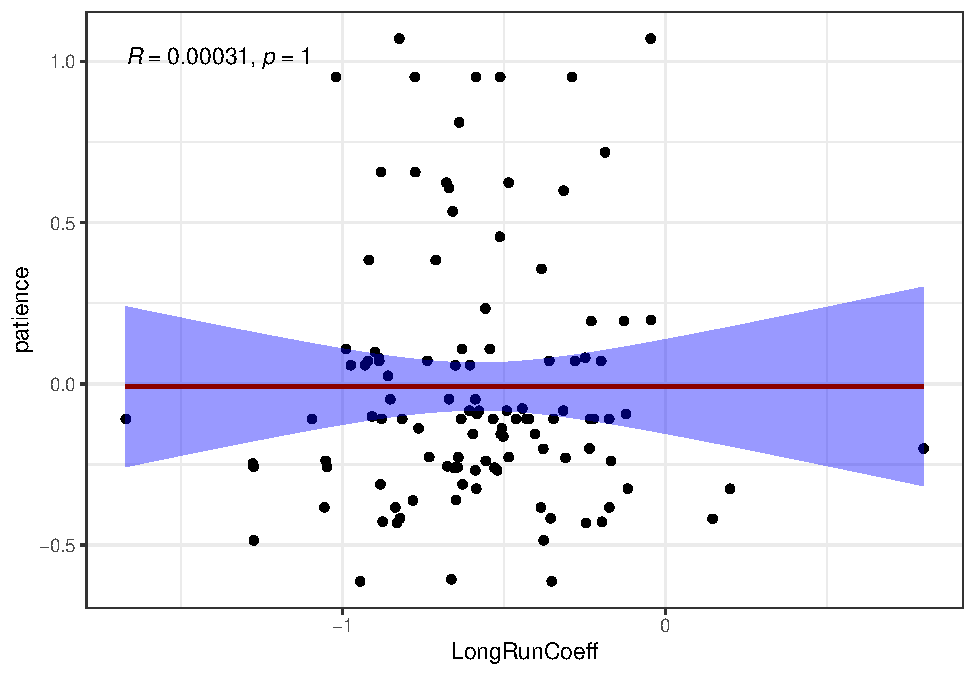
\includegraphics{LR_explore_OK_comms_files/figure-latex/covariates-3.pdf} 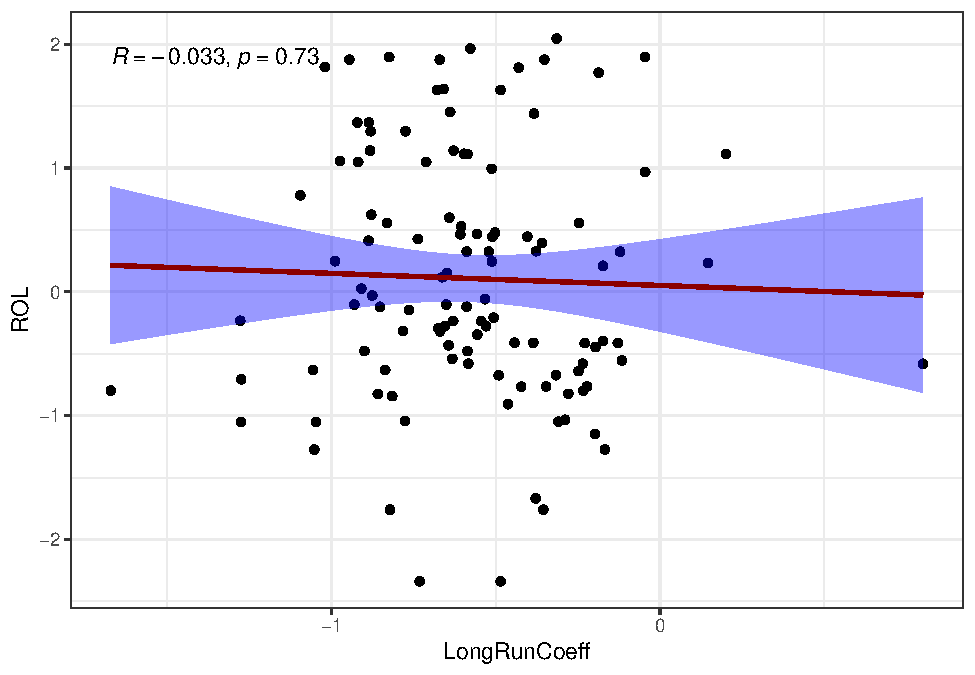
\includegraphics{LR_explore_OK_comms_files/figure-latex/covariates-4.pdf} 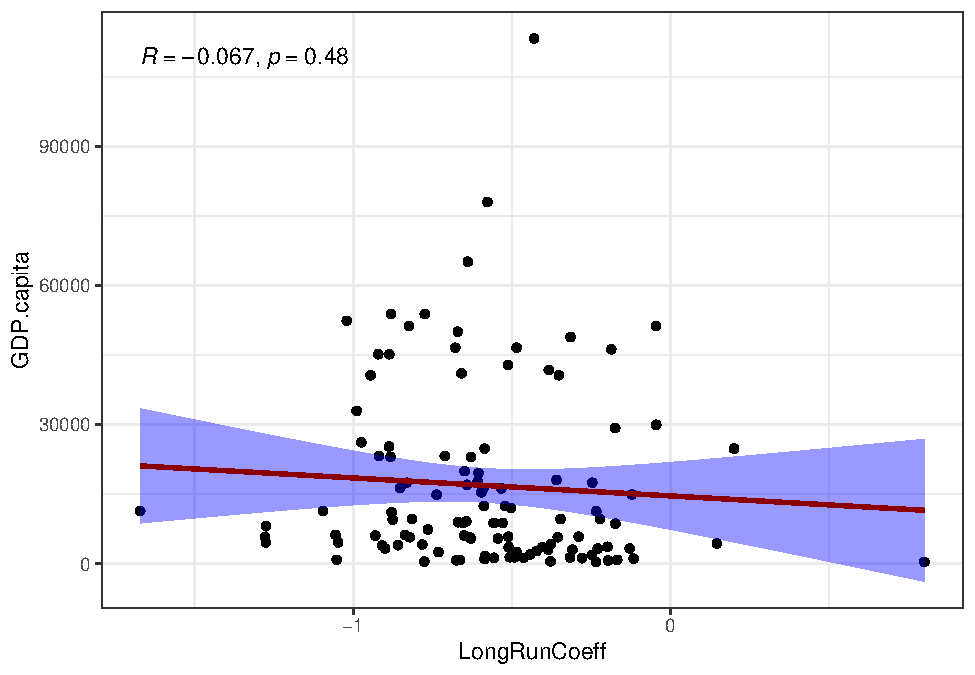
\includegraphics{LR_explore_OK_comms_files/figure-latex/covariates-5.pdf} 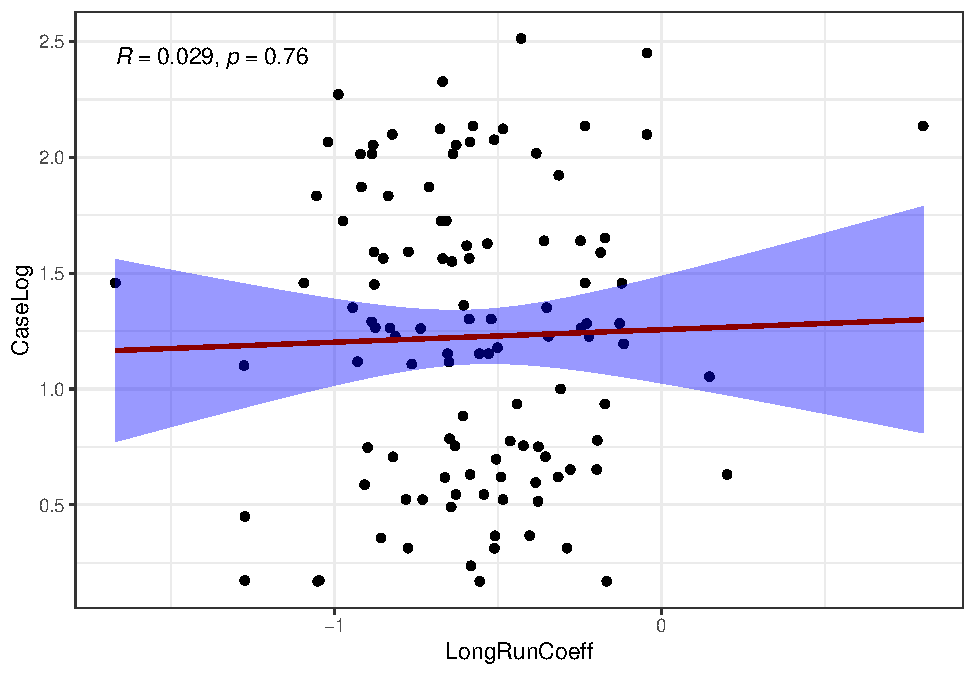
\includegraphics{LR_explore_OK_comms_files/figure-latex/covariates-6.pdf}

\end{document}
